\chapter{Environment}\label{ch:environment}

This chapter aggregates the previous information and introduces the Reinforcement Learning environment that simulates an initial circular orbit of a satellite in low earth orbit and an accelerated Orbital Decay. The initial conditions, the dynamics of the system, the action and observation space, a distributed optimization of PPO algorithm's hyper-parameter, an evaluation of PPO within this environment, and an analysis of the resulting PPO agent.

\section{Environment Description}

The dynamics of the environment follows that of the physics of Chapter~\ref{ch:physics}. The base of the environment revolves around Algorithm~\ref{alg:problemsim} using the 4th Order Yoshida integrator to calculate the next step's velocity and position from the previous velocity and position and the state's acceleration calculated from the gravitational force and the amplified Drag. 

One aspect of the Environment not yet described in Chapter~\ref{ch:physics} and Section~\ref{sec:reinforcement_learning} is how the satellite agent interacts with it's environment. The maximum force of propulsion of the satellite is a fraction of that of Ion Thruster at $0.04$ Newtons and, it being in a 2D-world or on a plane in a 3D-world, restricting its angle of thrust to a single degree of freedom with values between 0\si{\degree} and 360\si{\degree}. The agent operates in continuous action space with 2 values between 0 and 1. These two input values are not directly map to $[0, 0.04]$ for thrust and $[0, 360)$ as would be natural, but, to reduce variance, it is instead mapped to a delta of the thrust and angle values. This delta's range is $\frac{1}{50}$th the maximum thrust and $\frac{1}{6}$th the maximum angle. If the resulting value of the thrust after applying it's delta is greater than $0.04$ or less than $0$ it is clipped. On the other hand, the angle is wrapped to be between $-\pi$ and $\pi$ after applying the angle delta. The initial thrust is 0 and the initial thrust angle is normal to the origin. The height of the satellite is 550\si{km} from the surface or a radius of $6.921\times 10^6\si{meters}$. The mass of the satellite is 100\si{kg}, 75\si{kg} of which is propellant. Every step in the environment is equivalent to a second. The more massive object, to resemble earth has the same gravitational parameter, $3.986004418\times 10^{14}\si{m^3s^{-2}}$. The surface area of the satellite normal to the velocity is 1\si{m}, this is used while calculating the drag, while the drag coefficient is set to 2.123. As per Chapter~\ref{ch:physics}, the initial orbital velocity is $$v_{\text{orbital}}=\sqrt{\frac{GM}{r}}$$ where $GM$ is the gravitational parameter and $r$ is the radius from our stationary earth located at the origin. The force on the satellite is calculated using equation~\ref{eq:force} with a normal variation of 10\% of the force, but the density, $\rho$ in addition to using equation~\ref{eq:density} to initially calculate, it is multiplied by a hyper-parameter, $\xi$. With the termination threshold for the distance from the target orbit being 1\si{m}, the $\xi$ hyper-parameter is tuned so the density of the atmosphere results in an orbital decay where this termination threshold is reached in 200 steps, if no propulsion is used. The target of this agent in this environment is to maximize the number of steps within the termination threshold while having limited fuel. This means also minimizing the amount of fuel used.

To simplify the calculation of the remaining fuel and mass after each step, the satellite is given enough fuel for 125 steps at maximum thrust. A counter is kept that keeps track of the accumulated thrust before the mapping, which has the range $[0, 1]$. This accumulated thrust is then used to calculate if this threshold has been reached and remaining fuel mass. The mass of the satellite is also adjusted according to the remaining fuel, $$m_t=m_l+\bigg(1-\frac{\text{fuel used}}{\text{initial fuel}}\bigg)m_p.$$ Where $m_t$ is the mass at that step, $m_p$ is the mass of the propellant, and $m_l$ is the mass of the satellite without fuel.

The observation space is also continuous of size 8. It includes the normalized position with respect to the initial radius, normalized velocity with respect to the initial velocity, the euclidean distance between the satellite and the target orbit, the euclidean distance between the current velocity and the target velocity for the target circular orbit, the current angle, and the current thrust. All of these values are mapped to be between 0 and 1 before returning to them to the RL algorithm,
$$[r_x, r_y, v_x, v_y, r_{\text{targ}}, v_{\text{targ}}, \theta, F_{\text{thrust}}].$$
Where $r_{targ}=|||\vec{r}||_2 - r_\text{orbital}|$, $v_{\text{targ}}=|||\vec{v}||_2-v_\text{orbital}|$, $||x||_2$ is the euclidean norm operation, $|x|$ is the absolute value operation, $r_\text{orbital}$ is the starting radius, $\vec{r}$ is the current position of the satellite, and $\vec{v}$ is the current velocity of the satellite. The action space, as mentioned before, is continuous, has a size of 2, and includes the thrust delta and the angle delta, $$[\Delta F_{\text{thrust}}, \Delta \theta].$$ 

For every step, the reward signal consists of the current step of the environment divided by 800 plus 0.5 and if the agent either crosses the orbital termination threshold or if it runs out of fuel the episode ends with 0 reward for that step. This linear increase of the reward per step encourages the agent to both not run out of fuel and stay within the orbital termination threshold. \begin{equation}\label{eq:reward}
r_t = \begin{cases}
	0 & \mbox{if }r_{\text{targ}}>r_{\text{threshold}}\lor f_{\text{used}}>f_{\text{available}} \\
	\frac{t_{\text{step}}}{800} + 0.5 & \mbox{otherwise}
\end{cases}
\end{equation}
Where $r_{\text{targ}}$ is the distance from the target orbit, $r_{\text{threshold}}$ is the threshold, $f_{\text{used}}$ is the amount of fuel used, $f_{\text{available}}$ is the amount of fuel available, and $t_{\text{step}}$ is the number of steps since the start of the episode. If the environment's episode reaches 800 steps it is ended. 

\begin{figure}
	\centering
	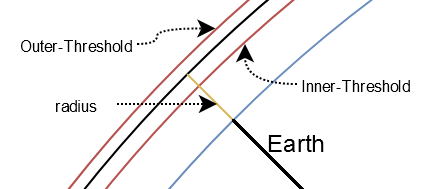
\includegraphics{OrbitDiagram}
	\caption{A diagram of the target orbit and the termination orbital threshold.}
	\label{fig:OrbitDiagram}
\end{figure}

Normally calculating the acceleration, the velocity and position using the 4th order yoshida integrator is computationally expensive, especially because the language, python, used is not a compiled language. This is mitigated using the Numba \cite{10.1145/2833157.2833162} library. Using Numba, the portion of the code that calculates the acceleration and calculates the 4th order yoshida integration are compiled using a Just-in-time (JIT) compiler.

The python Reinforcement Learning library stable-baselines' PPO algorithm implementation was used. stable-baseline is a fork of the baseline library created OpenAI and improves upon it. It uses the PPO-Clip variant of the PPO algorithm.

The environment is built on-top of the python framework laid out by the OpenAI's Gym \cite{DBLP:journals/corr/BrockmanCPSSTZ16}. All of Gym's environment, including this environment, inherit their Env object which lays out a standard set of functions to override when creating an environment that inherently works with most Reinforcement Learning libraries out there. The functions to override includes the seed function that generates a random seed or takes in a seed from the user, the reset function that resets the environment and is run between episodes, it returns the initial observation of the environment, the step function that moves the environment a single step forward, which takes in the actions to take and returns the next step's observed state, it's reward, and whether the episode has reached termination. The step function can be seen in pseudo-code form in Algorithm~\ref{algo:step}.

\begin{algorithm}\label{algo:step}
	\SetAlgoLined
	\DontPrintSemicolon
	\KwIn{Input action tuple $(a_1, a_2)$, both values of which are between 0 and 1.}
	\KwData{The satellite's last position $\vec{r}$, velocity $\vec{v}$, thrust $t$, angle $\theta$, and fuel used $f_{\text{used}}$.}
	$\text{thrust}\leftarrow \text{clip}(t + 0.04 a_1 - 0.02, 0.0, 1.0)$\\
	$\theta\leftarrow \text{wrap}(\theta + \frac{\pi a_2}{3}-\frac{\pi}{6})$\\
	$\vec{r}, \vec{v}\leftarrow$calculate\_physics$(\vec{r}, \vec{v}, \text{thrust}, \theta)$\\
	$r_{\text{targ}}=|||\vec{r}||_2-r_{\text{orbital}}|$ \\
	$v_{\text{targ}}=|||\vec{v}||_2-v_{\text{orbital}}|$ \\
	$f_{\text{used}}\leftarrow f_{\text{used}}+t$\\
	$m\leftarrow m_f+\big(1-\frac{f_{\text{used}}}{f_{\text{available}}}\big)m_p$\\
	reward$=$Equation~\ref{eq:reward}\\
	done$\leftarrow r_{\text{targ}}>$threshold$\lor f_{\text{used}}>$fuel threshold\\
	\Return $\vec{r}, \vec{v}, r_{\text{targ}}, v_{\text{targ}}, \theta, t,$reward, done
	\caption{Calculate the environment's next step.}
\end{algorithm}
	
\section{Hyper-parameters \& Distributed Hyper-parameter Optimization}

Here, Optuna \cite{DBLP:journals/corr/abs-1907-10902} was used to optimize the PPO hyper-parameter. Optuna is a hyper-parameter optimization framework that automates the hyper-parameter search. Unfortunately, due to the large number of hyper-parameters the search space is very large and difficult to search with one machine. To mitigate this the distributed feature of Optuna was used.

This Optuna feature involves creating a MySQL server which is then used by the workers to coordinate the optimization. A MySQL management service was created called OptunaExplorer to dynamically interact and manage the MySQL server as the workers optimize. A run when optimizing is called a trial and a set of trials to optimize a problem is called a study, in Optuna. The study to optimize the PPO hyper-parameters for this environment ran for 536 trials using 9 workers spread evenly across 3 computers utilizing GPU acceleration.

The optimized hyper-parameters include the lambda, or the GAE parameter used to control the balance between bias and variance, $\gamma$ or the discount factor from equation~\ref{eq:discountedreward}, the learning rate which is used with the Adam Optimizer used to train the algorithm, the Entropy Coefficient, $c_1$ from equation~\ref{eq:PPO_objective}, is used to prevent premature convergence, and the Clipping parameter, $\epsilon$ from equation~\ref{eq:PPO_clip_objective}. The rest of the parameters were not explicitly optimized. 

\begin{table}
	\begin{tabularx}{\columnwidth}{|c|c|X|} \hline
		Hyper-parameter & Value & Description \\\hline\hline
		$\gamma$ & $0.994404$ & Discount Factor\\\hline
		$n_{\text{steps}}$ & 256 & Number of steps for each environment update. \\\hline
		$c_1$ & 0.00377952 & Entropy Coefficient \\\hline
		Learning rate & 0.000819363 & Used with the Adam Optimizer \\\hline
		$c_2$ & 0.5 & Value function coefficient used with equation~\ref{eq:PPO_objective}. \\\hline
		Gradient Clipping & 0.5 & Limits weight changes when updating Neural Networks. \\\hline
		$\lambda$ & 0.944959 & GAE Coefficient \\\hline
		$n_{\text{minibatches}}$ & 8 & Number of mini-batches to train for per update. \\\hline
		$n_{\text{opteochs}}$ & 4 & Epochs to train surrogate \\\hline
		$\epsilon$ & 0.0343517 & Clipping parameter from equation~\ref{eq:PPO_clip_objective} \\\hline
	\end{tabularx}
	\caption{The PPO hyper-parameters used for the environment introduced.}\label{table:ppo_parameters}
\end{table}

\section{Methodology, Training, \& Evaluation}

PPO was trained for 10,000,000 steps using the parameters from Table~\ref{table:ppo_parameters} 7 times with different seeds, thereby generating 7 different training trajectories. The parameter from Table~\ref{table:ppo_parameters} were generated using distributed optimization with Optuna and OptunaExplorer. The episode reward, the advantage, and the discounted rewards were recorded during training. For every 5000 training steps the model is evaluated for 100 episodes where the average and standard deviation of the episode reward are aggregated and recorded. The 7th run's best model is saved for later evaluation. The training metrics are stored via TensorBoard then converted to CSV format via a custom callback that outputs a plot and CSV file of the accumulated data. All current and historical data and code is available though the GitHub page, \href{https://github.com/anhydrous99/Thesis}{https://github.com/anhydrous99/Thesis}.

PPO2 from the stable-baselines library was used which is a parallel implementation of the PPO-Clip algorithm. In it's source code it is called "GPU version" due to it's parallel nature and it's improved efficiency within GPUs. The stable-baselines library is build atop Google's Tensorflow 1.x library, a popular Machine Learning library.

\begin{table}
	\centering
	\begin{tabular}{|c|c|} \hline
		Run & Best Model Reward \\\hline\hline
		1 & 451.468 \\\hline
		2 & 455.328 \\\hline
		3 & 450.521 \\\hline
		4 & 385.410 \\\hline
		5 & 448.616 \\\hline
		6 & 400.421 \\\hline
		7 & 421.122 \\\hline
	\end{tabular}
	\caption{ The best model's average reward per run. This average reward is calculated over 100 episodes. }\label{table:best_evaluation_rewards}
\end{table}

\begin{figure}
	\centering
	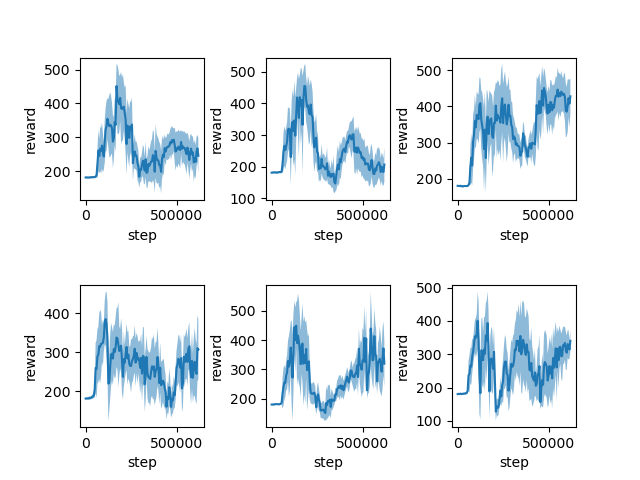
\includegraphics{TestPlot}
	\caption{Six plots, one for each training run excluding the last run, showing the results of the evaluation steps.}
	\label{fig:validation_runs}
\end{figure}

\begin{figure}
	\centering
	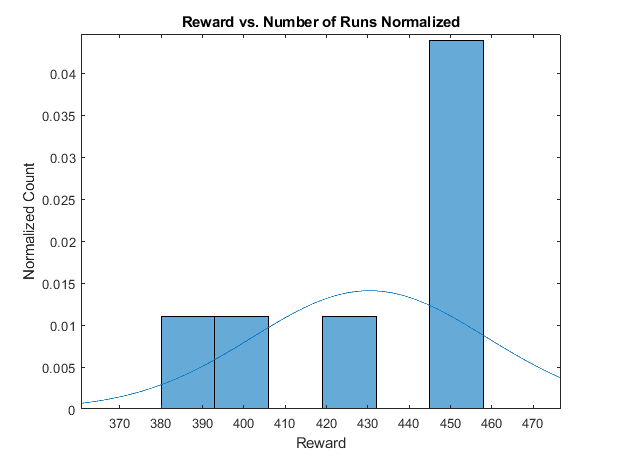
\includegraphics{RewardvRunsNormalized}
	\caption{A histogram and normal fit of the data on Table~\ref{table:best_evaluation_rewards} where the x-axis has been separated into 6 bins from the maximum reward to the minimum reward. The y-axis is the number of occurrences of said reward normalized. The fitted normal probability has $\mu=430.411$ and $\sigma=28.3151$.}
	\label{fig:norm_hist_reward}
\end{figure}

\begin{figure}
	\centering
	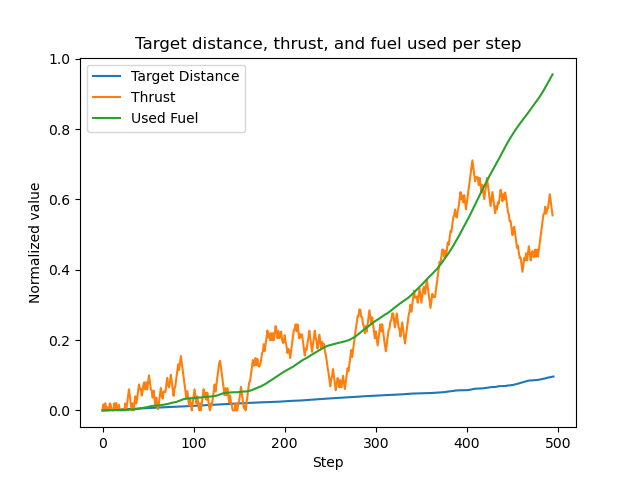
\includegraphics{TargetDistanceThrustUsedFuel}
	\caption{A plot of an episode generated from the 7th run's best model. The distance from the target orbit, the satellite's thrust, and the amount of used fuel are normalized between 0 and 1 then plotted.}
	\label{fig:tdtuf}
\end{figure}

\section{Discussion}

It was possible to train the PPO agent to be successful by reaching a reward of above 400 but only about 1/6th of the time. Meaning, there is still room to grow and develop an agent that is able to achieve higher reward at a more consistent rate. 